\section{Hidden Portal}\label{section:HiddenPortal}

\subsection{The first look}
The UART status message reported a \texttt{wifi\_clients} counter, and the firmware strings mentioned a SoftAP, so we looked for a Wi-Fi access point. The network was visible nearby, with a BSSID right next to the device MAC (\texttt{B8:D6:1A:4C:48:64}):

\begin{lstlisting}
$ nmcli device wifi list | grep GW
B8:D6:1A:4C:48:65  SmartHomeGW_4C4864  Infra  11  ...  WPA2
\end{lstlisting}

The Wi-Fi password, \texttt{gateway-secure-2026}, was shown on the device display. After connecting, the gateway log confirmed it with \texttt{Client connected to SoftAP}, and \texttt{wifi\_clients} went up to 1.

\subsection{The web dashboard}
The firmware strings also mentioned a web dashboard on port 80. Opening \texttt{http://192.168.4.1} showed the gateway dashboard with a PIN entry page, a log terminal and a UDP broadcast button (Figure~\ref{fig:portal-dashboard}).

\begin{figure}[htbp]
  \centering
  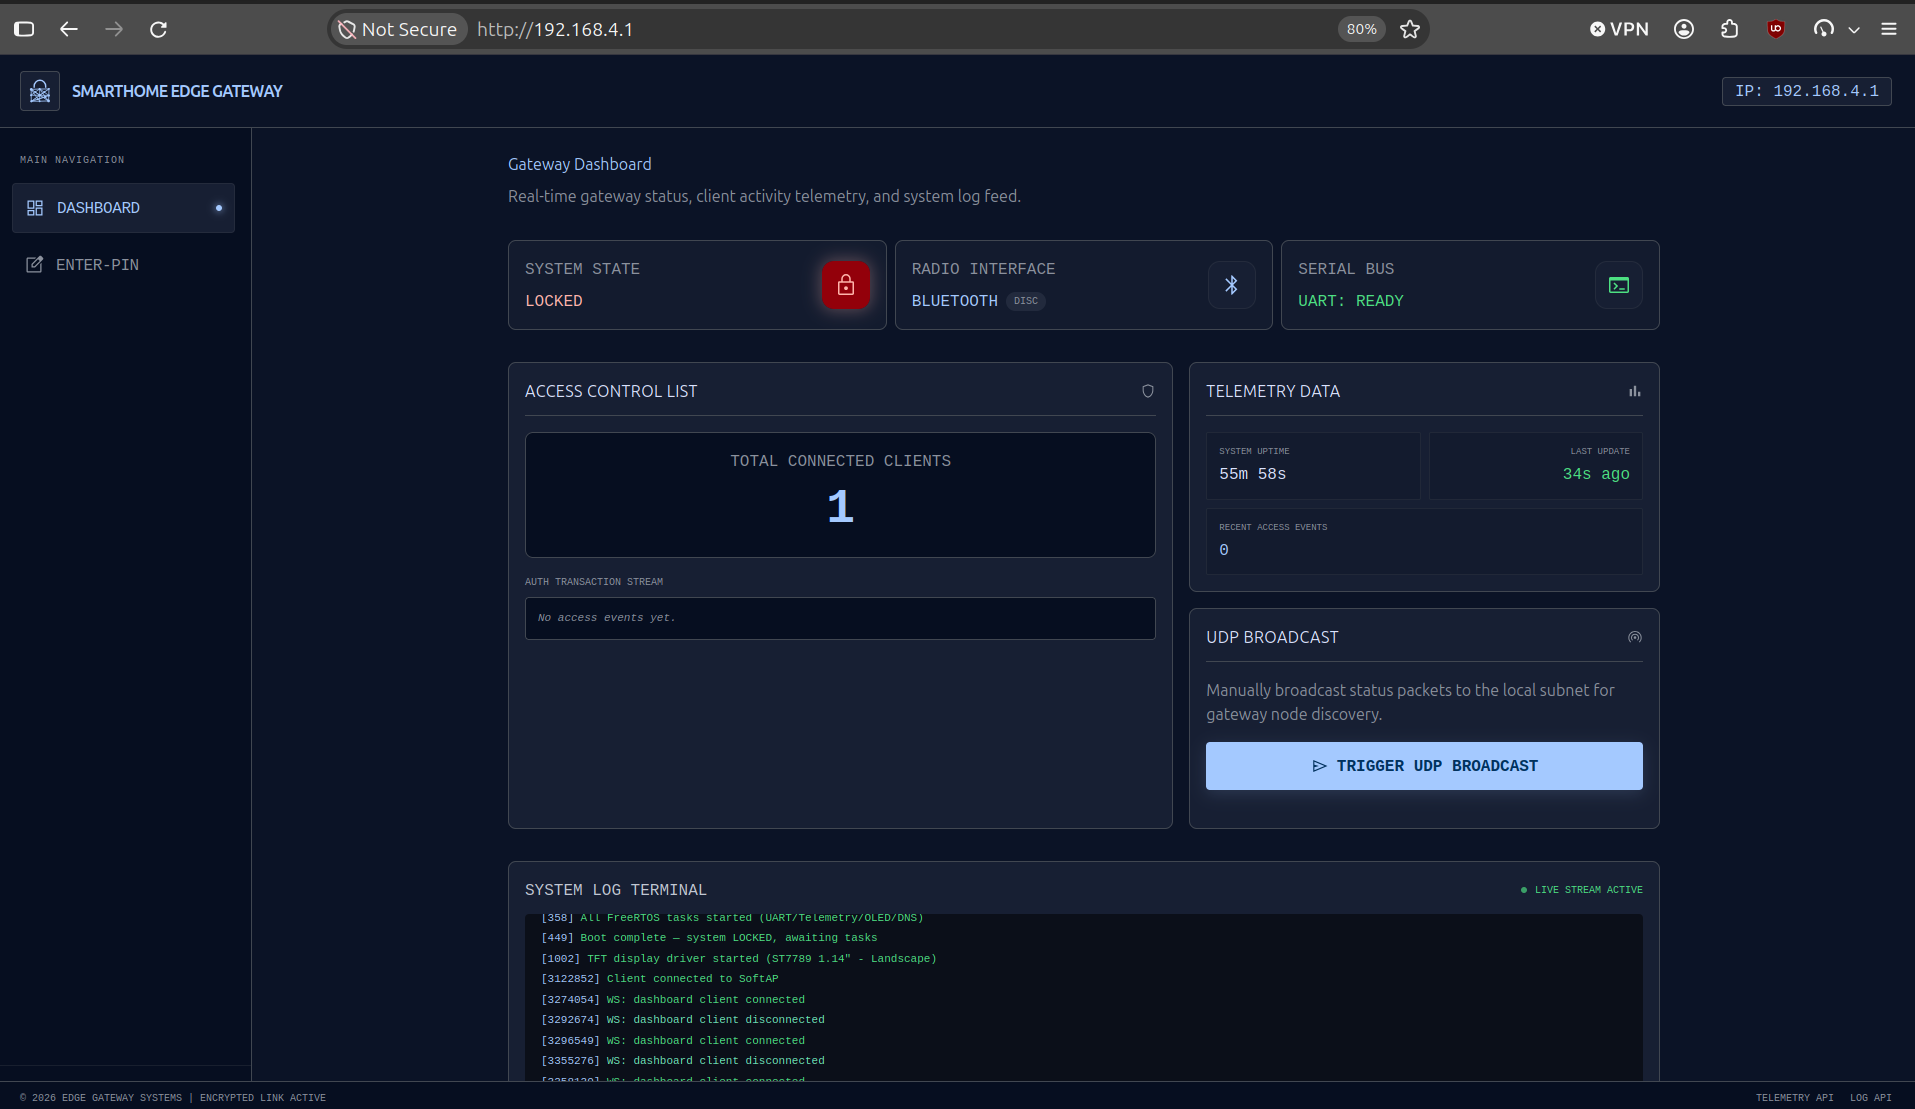
\includegraphics[width=0.8\columnwidth]{4-smarthome-webpage.png}
  \caption{The SmartHome gateway dashboard at \texttt{192.168.4.1}.}
  \label{fig:portal-dashboard}
\end{figure}

The log (\texttt{/api/log?since=0}) showed a telemetry task broadcasting on UDP port 4210. Capturing these broadcasts revealed one extra field that the UART status did not have:

\begin{lstlisting}[basicstyle=\ttfamily\scriptsize]
$ sudo tcpdump -ni wlp0s20f3 -A 'udp and src host 192.168.4.1 and port 4210'
{"event":"status_update", ... ,"recent_access":[],"dev_dashboard":"/api/admin"}
\end{lstlisting}

\subsection{Finding the PIN}
The hidden \texttt{/api/admin} page showed a ``diagnostic carrier asset'', a small $64\times48$ picture available for download (Figure~\ref{fig:portal-admin}). Its PNG metadata had \texttt{Comment: steganography}, so we ran \texttt{zsteg} on it and found the PIN in the least significant bits of the red channel:

\begin{lstlisting}
$ zsteg -a admin.png
meta Comment        .. text: "steganography"
b1,r,lsb,xy         .. text: "PIN:4390"
\end{lstlisting}

\begin{figure}[htbp]
  \centering
  
\includegraphics[width=0.3\columnwidth]{admin.png}
  \caption{\texttt{admin.png}, the carrier image from \texttt{/api/admin}.}
  \label{fig:portal-admin}
\end{figure}

\subsection{The vault}
Entering the PIN opened \texttt{/vault} with an encoded payload and a hint: \emph{``50 shades of grey? 256 would've been better...''}

\begin{lstlisting}[basicstyle=\ttfamily\scriptsize]
4b4f59304e5c5d4a3052585b5b515956305d59304f514b4e304e583054
574e304e5c5730555a51542730565d515470564f5b483069615f647b52
\end{lstlisting}

``Grey'' with 256 values pointed to 8-bit Gray code. Decoding each byte from Gray code back to binary (script \texttt{gray.py}) gave:

\begin{lstlisting}[basicstyle=\ttfamily\scriptsize]
run this command in uart to get the flag: diag_dump NAjGRc
\end{lstlisting}

Sending this command over UART returned the flag:

\begin{lstlisting}[basicstyle=\ttfamily\scriptsize]
Diagnostic dump authorized. Flag: esc_2026{50_shades_of_grey_77a7d0147d862881}
\end{lstlisting}

\begin{center}
\fbox{\texttt{esc\_2026\{50\_shades\_of\_grey\_77a7d0147d862881\}}}
\end{center}
